\documentclass{article}
\usepackage{graphicx} % Required to insert images

\usepackage{fullpage}

\usepackage{hyperref}

\pagestyle{empty}
%
%\usepackage{caption}
%\captionsetup{labelformat=empty}

% --- Document Start ---
\begin{document}

% This command prevents the figure environments from being numbered.
\renewcommand{\thefigure}{}

\large{\textbf{Examples of \url{https://github.com/QiDawei98/Flower_Lane}:}

% --- Top Row of Images ---
% The 'figure' environment is a container for floating content like images.
% The [h!] option suggests that LaTeX place the figure "here" if possible.
\begin{figure}[h!]
    \centering % This centers the images on the page.
    
    % The 'minipage' environment creates a small, independent page area.
    % We create two, each taking up slightly less than half the page width
    % to leave a small margin between them.
    \begin{minipage}{0.48\textwidth}
        \centering
        % Replace 'image1.png' with your first image file.
        % The [width=\linewidth] option scales the image to fit the minipage.
        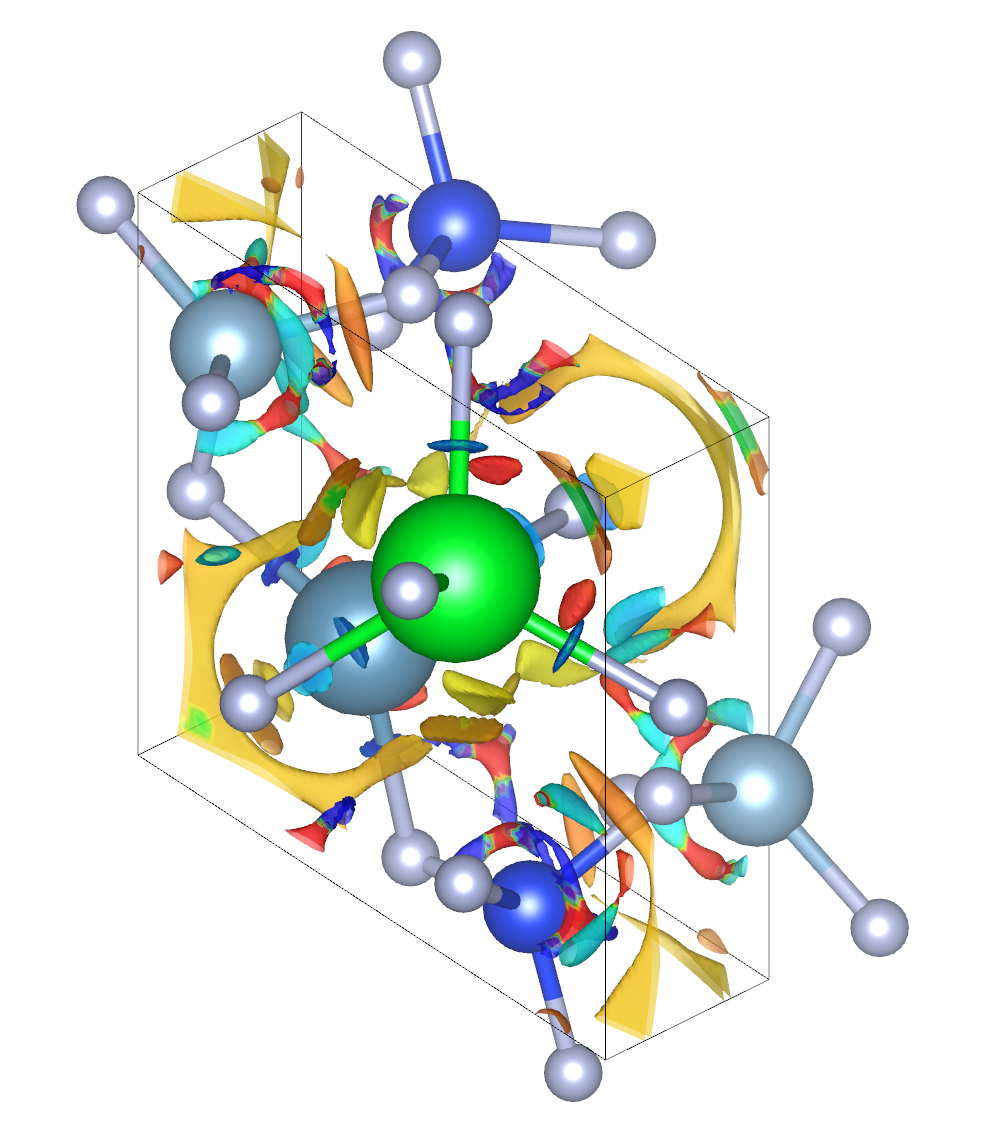
\includegraphics[width=0.9\linewidth]{1}
    \end{minipage}
    \hfill % This command creates a flexible horizontal space between the two minipages.
    \begin{minipage}{0.48\textwidth}
        \centering
        % Replace 'image2.png' with your second image file.
        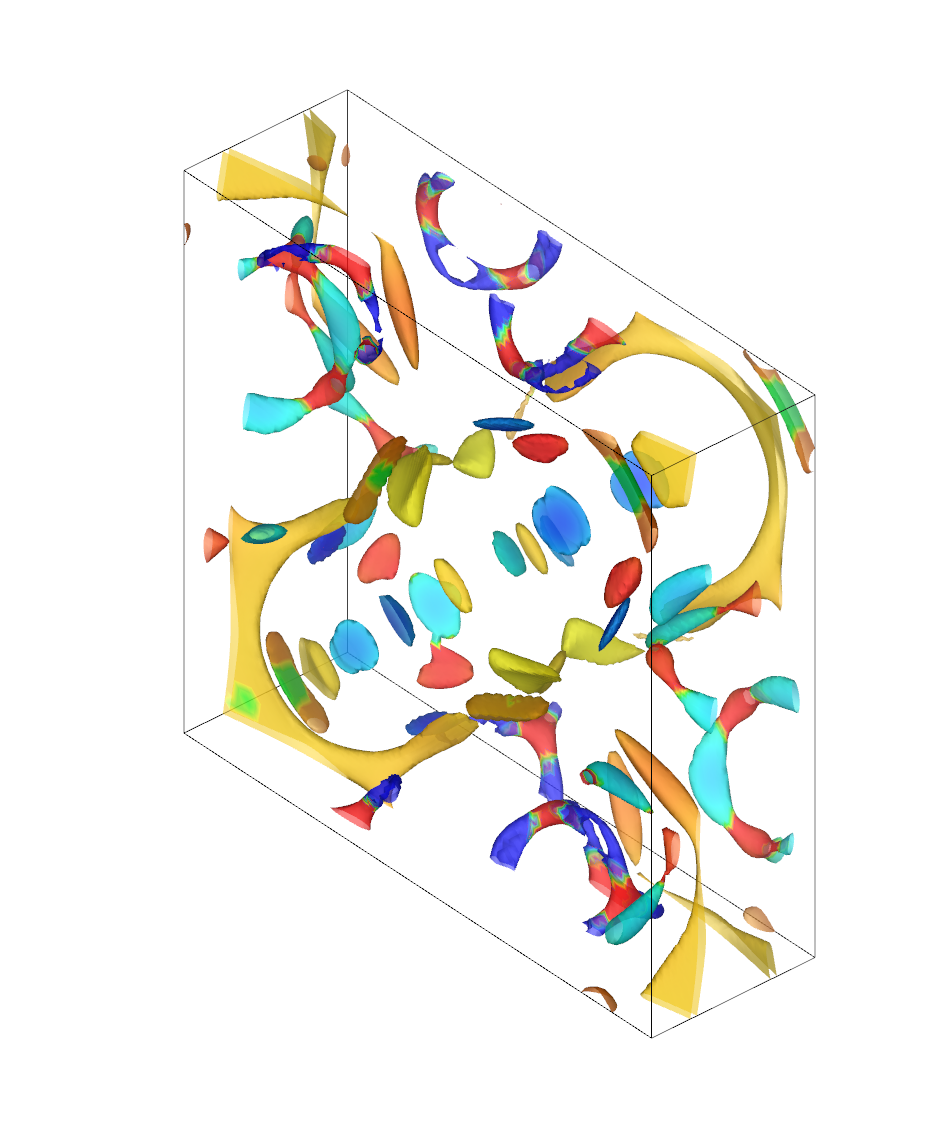
\includegraphics[width=0.9\linewidth]{2}
    \end{minipage}
    
    \caption{mp-1235507  BaSrLiNdTlCu2O7}
    
\end{figure}


% --- Bottom Row of Images ---
% We repeat the same structure for the second row of images.
\begin{figure}[h!]
    \centering
    
    \begin{minipage}{0.48\textwidth}
        \centering
        % Replace 'image3.png' with your third image file.
        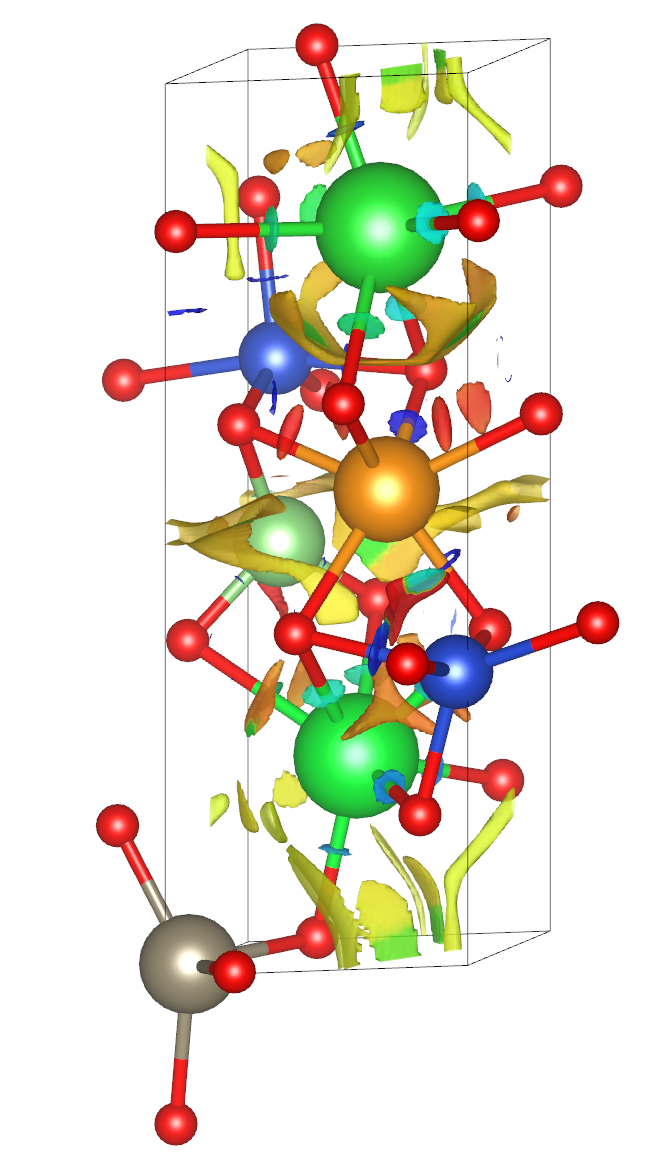
\includegraphics[scale=0.4]{3}
    \end{minipage}
    \hfill
    \begin{minipage}{0.48\textwidth}
        \centering
        % Replace 'image4.png' with your fourth image file.
        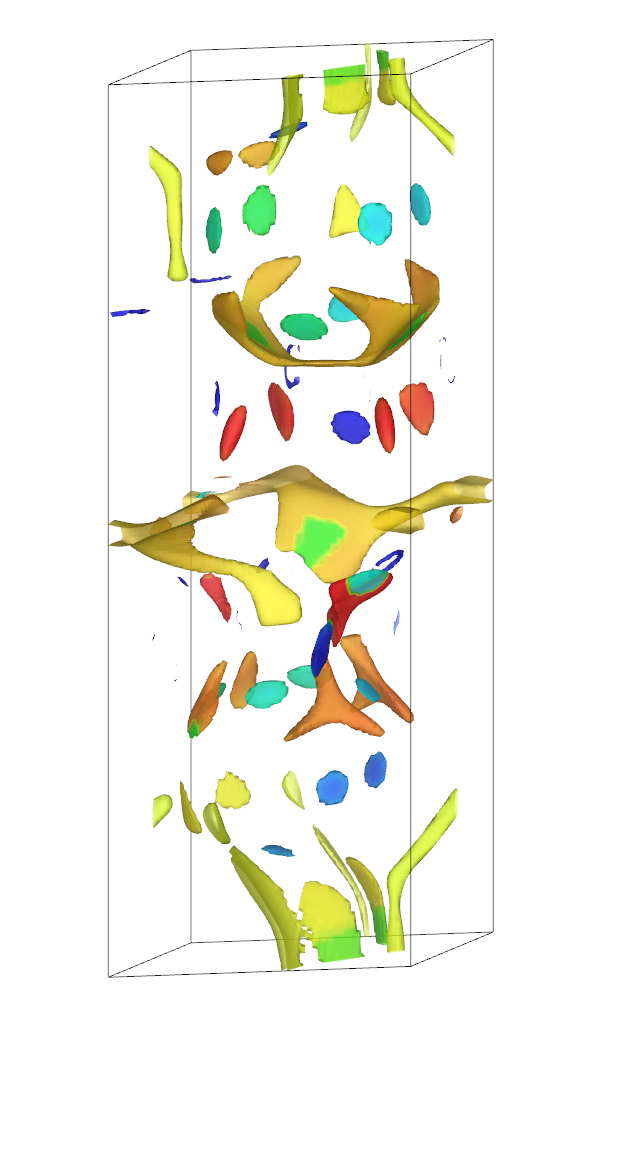
\includegraphics[scale=0.4]{4}
    \end{minipage}
    
    \caption{mp-1218409  SrCaAl2(SiN3)2}
    
\end{figure}

% --- Document End ---
\end{document}
